\documentclass[border=0pt]{standalone}
\usepackage{amsmath,amssymb}
\usepackage{xcolor}
\usepackage{tikz}
\renewcommand{\sfdefault}{phv}
\usetikzlibrary{arrows.meta,fit,shapes.symbols,shapes.geometric,positioning,calc}
% --- reusable vector icons for the system-view figure ---
% figure lettering: 8 pt Helvetica, the journal's minimum (the class's \footnotesize is only 7 pt)
\newcommand{\figfont}{\sffamily\fontsize{8}{9.6}\selectfont}
\newcommand{\gnbtower}[1]{%
  \begin{scope}[shift={#1}]
    \draw[thick,gray!45!black,fill=gray!12] (-0.15,0)--(0,0.82)--(0.15,0)--cycle;
    \draw[gray!55!black] (-0.095,0.28)--(0.095,0.28) (-0.065,0.46)--(0.065,0.46) (-0.035,0.63)--(0.035,0.63);
    \fill[gray!55] (-0.12,0.64) rectangle (-0.03,0.84);
    \fill[gray!55] (0.03,0.64) rectangle (0.12,0.84);
    \draw[blue!55!black] (0.17,0.72) arc (-55:55:0.13);
    \draw[blue!55!black] (0.22,0.68) arc (-55:55:0.21);
    \draw[blue!55!black] (-0.17,0.72) arc (235:125:0.13);
    \draw[blue!55!black] (-0.22,0.68) arc (235:125:0.21);
  \end{scope}
}
\newcommand{\uephone}[2]{%
  \begin{scope}[shift={#1}]
    \draw[thick,#2!65!black,fill=#2!14,rounded corners=1pt] (-0.12,-0.2) rectangle (0.12,0.2);
    \fill[#2!30] (-0.08,-0.09) rectangle (0.08,0.13);
    \fill[#2!65!black] (0,-0.15) circle (0.016);
  \end{scope}
}

\begin{document}
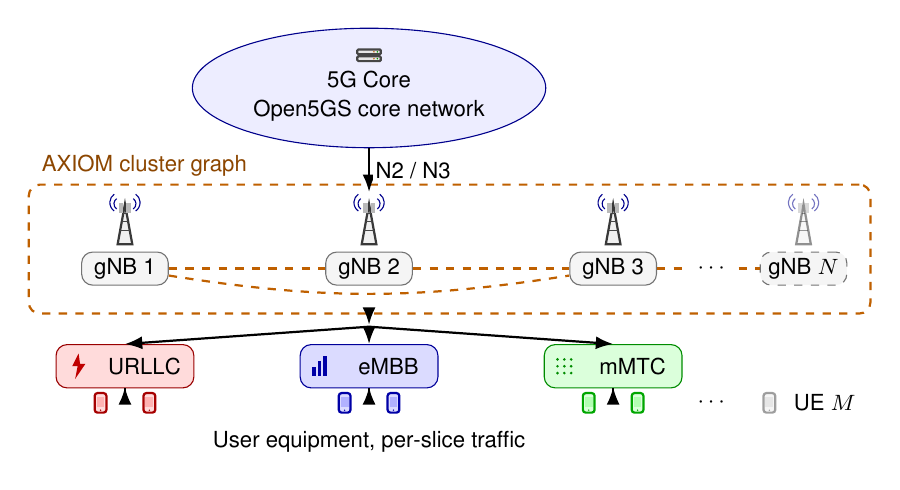
\begin{tikzpicture}[x=0.62cm,y=0.62cm,
  font=\figfont,
  core/.style={draw=blue!55!black, fill=blue!7, ellipse,
               minimum width=3.4cm, minimum height=1.1cm, align=center},
  gnb/.style={draw=black!55, rounded corners, fill=gray!8, minimum width=1.1cm,
              minimum height=0.42cm, align=center, font=\figfont, inner sep=1pt},
  band/.style={draw, rounded corners, minimum width=1.75cm, minimum height=0.55cm},
  ar/.style={-{Latex[length=2.2mm]}, thick},
  gedge/.style={dashed, thick, draw=orange!75!black}
]
% --- 5G Core (cloud-like ellipse) with a small server-rack glyph ---
\node[core] (core) at (7.5,6.75) {\\[2pt]{\figfont 5G Core}\\[1pt]{\figfont Open5GS core network}};
\begin{scope}[shift={(7.5,7.3)}]
  \foreach \yy in {0,0.14}{
    \draw[thick,gray!55!black,fill=gray!18,rounded corners=0.4pt] (-0.24,\yy) rectangle (0.24,\yy+0.1);
    \fill[green!60!black] (0.17,\yy+0.05) circle (0.017);
    \fill[orange!75!black] (0.10,\yy+0.05) circle (0.017);
  }
\end{scope}
% --- gNB towers + labels ---
\foreach \x/\i in {2.5/1,7.5/2,12.5/3}{
  \gnbtower{(\x,3.55)}
  \node[gnb] (g\i) at (\x,3.05) {gNB~\i};
}
\draw[gedge] (g1) -- (g2);
\draw[gedge] (g2) -- (g3);
\draw[gedge] (g1) to[bend right=9] (g3);
% --- further gNBs: the cluster holds N of them (7, 19, or 37 in the scaling study) ---
\node[font=\figfont] (gdots) at (14.55,3.05) {$\cdots$};
\begin{scope}[opacity=0.55]\gnbtower{(16.4,3.55)}\end{scope}
\node[gnb, dashed] (gN) at (16.4,3.05) {gNB~$N$};
\draw[gedge] (g3) -- (gdots); \draw[gedge] (gdots) -- (gN);
\node[draw=orange!75!black, dashed, thick, rounded corners, inner sep=3pt,
      fit={(0.7,2.3) (17.6,4.6)}] (clu) {};
\node[font=\figfont, text=orange!55!black, inner sep=1.5pt]
      at (0.7,4.85) [anchor=south west] {AXIOM cluster graph};
\draw[ar] (core.south) -- (7.5,4.62) node[pos=0.5, right=1pt, font=\figfont, fill=white, inner sep=1pt] {N2 / N3};
% --- slice bands with icons + short labels ---
\node[band, fill=red!14,   draw=red!60!black]   (s1) at (2.5,1.05) {};
\node[band, fill=blue!14,  draw=blue!60!black]  (s2) at (7.5,1.05) {};
\node[band, fill=green!14, draw=green!55!black] (s3) at (12.5,1.05) {};
\node[font=\figfont] at (2.9,1.05) {URLLC};
\node[font=\figfont] at (7.9,1.05) {eMBB};
\node[font=\figfont] at (12.9,1.05) {mMTC};
% URLLC bolt
\fill[red!75!black] (1.55,1.31)--(1.42,1.05)--(1.53,1.05)--(1.48,0.79)--(1.69,1.10)--(1.58,1.10)--cycle;
% eMBB bandwidth bars
\fill[blue!65!black] (6.34,0.85) rectangle (6.41,1.03);
\fill[blue!65!black] (6.45,0.85) rectangle (6.52,1.15);
\fill[blue!65!black] (6.56,0.85) rectangle (6.63,1.27);
% mMTC sensor grid
\foreach \a in {-0.14,0,0.14}{\foreach \b in {-0.14,0,0.14}{\fill[green!55!black] (11.5+\a,1.05+\b) circle (0.03);}}
\draw[ar] (g2 |- clu.south) -- (7.5,1.9);
\draw[ar] (7.5,1.86) -- (s1.north);
\draw[ar] (7.5,1.86) -- (s2.north);
\draw[ar] (7.5,1.86) -- (s3.north);
% --- UEs ---
\uephone{(2.0,0.3)}{red}  \uephone{(3.0,0.3)}{red}
\uephone{(7.0,0.3)}{blue} \uephone{(8.0,0.3)}{blue}
\uephone{(12.0,0.3)}{green} \uephone{(13.0,0.3)}{green}
\node[font=\figfont] at (14.55,0.3) {$\cdots$};
\begin{scope}[opacity=0.55]\uephone{(15.7,0.3)}{gray}\end{scope}
\node[font=\figfont, anchor=west] at (16.0,0.3) {UE~$M$};
\node[font=\figfont] at (7.5,-0.5) {User equipment, per-slice traffic};
\draw[ar] (s1.south) -- (2.5,0.62);
\draw[ar] (s2.south) -- (7.5,0.62);
\draw[ar] (s3.south) -- (12.5,0.62);
\end{tikzpicture}
\end{document}
